%@+leo-ver=5-thin
%@+node:jegc.20110930171547.1123: * @file alternativa.tex
%@@language latex

\documentclass{beamer}

%@+<<tema de beamer>>
%@+node:jegc.20110930171547.1114: ** <<tema de beamer>>
\useinnertheme[shadow=true]{rounded}
\useoutertheme{infolines}
\usecolortheme{orchid}
\definecolor{rojo}{rgb}{0.9,0,0}
\setbeamercolor{structure}{fg=rojo}
\setbeamercolor{item projected}{use=item,fg=black,bg=item.fg!50}
\setbeamercolor*{palette primary}{fg=white,bg=rojo}
\setbeamercolor*{palette secondary}{parent=palette primary,use=palette primary,bg=palette primary.bg!90!black}
\setbeamercolor*{palette tertiary}{parent=palette primary,use=palette primary,bg=palette primary.bg!80!black}
\setbeamercolor*{palette quaternary}{parent=palette primary,use=palette primary,bg=palette primary.bg!70!black}
\setbeamercolor{titlelike}{parent=palette primary}
\setbeamercovered{highly dynamic}
%@-<<tema de beamer>>

\usepackage[utf8]{inputenc}
\usepackage[spanish]{babel}
\usepackage{graphicx}
\usepackage{url}
\usepackage{times}
\usepackage[T1]{fontenc}
\hypersetup{pdfkeywords=open free design source hardware colombia Software Libre abierto 2011 AltaImpedancia alta impedancia electrónica alternativa simulación simulation circuit circuito}

\title[Simulación de circuitos con Software Libre]{Simluación de circuitos con Software Libre}
\author[JEGC 2011]{Jorge~Ernesto~Guevara~Cuenca}
\institute[\url{www.fuac.edu.co}]
{ \inst{1}
  Colibri - Comunidad de Usuarios de Software Libre en Colombia\\
  \url{http://www.slcolombia.org}
  \and
  \inst{2}
  Alta Impedancia - \url{http://www.altaimpedancia.org}
  \and
  \inst{3}
  Hackbo - Hackerspace Bogotá -  \url{http://www.hackbo.co}
  \and
  \inst{4}
  Universidad Autónoma de Colombia - \url{http://www.fuac.edu.co}
}
\date[III Muestra tecnológica UAC]
{III Muestra tecnológica\\Universidad Autónoma de Colombia\\26 de octubre de 2011}

\subject{Simulación de circuitos con Sofware Libre, III Muestra tecnológica Universidad Autónoma de Colombia, 26 de octubre de 2011}


\logo{
\includegraphics[height=1cm]{img/uac}}

\AtBeginSubsection[]
{ \begin{frame}<beamer>{Agenda}
    \tableofcontents[currentsection,currentsubsection]
  \end{frame}}

\beamerdefaultoverlayspecification{<+->}

\begin{document}

\begin{frame}
  \titlepage
\end{frame}

\begin{frame}
  \frametitle{Agenda}
  \tableofcontents
  % You might wish to add the option [pausesections]
\end{frame}

\section<presentation>*{Simulación de circuitos con Software Libre}

\begin{frame}
  \frametitle{Objetivos}
  \begin{itemize}
  \item Dar a conocer algunas aplicaciones de Software Libre EDA.
  \item Incentivar el uso de Software Libre para electrónica en la educación.
  \item Mostrar como simular circuitos electricos mediante ejemplos con los programas qucs, scilab y gEDA con gnucap.
  \end{itemize}
\end{frame}

\section{Proyectos de Open Source Hardware}

\subsection{Motivación}

\begin{frame}{IP04 IP-PBX}{\url{http://www.rowetel.com}}
  \begin{figure}
    \centering
    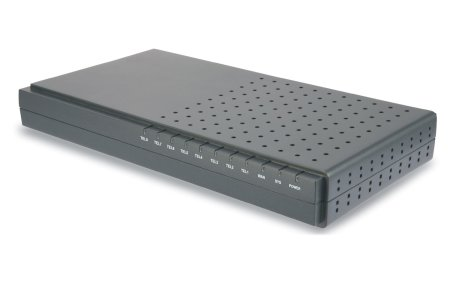
\includegraphics{img/ip04}
    \caption{PBX IP 4 puertos (Asterisk)}
    \label{fig:asterisk}
  \end{figure}
\end{frame}

\begin{frame}{Arduino}{\url{http://www.arduino.cc}}
  \begin{figure}
    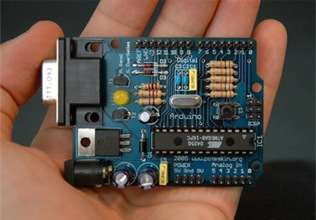
\includegraphics[scale=0.6]{img/arduino316}
    \caption{Plataforma para prototipado.}
    \label{fig:arduino}
  \end{figure}
\end{frame}

\begin{frame}{Wiring}{\url{http://wiring.org.co}}
  \begin{figure}
    \centering
    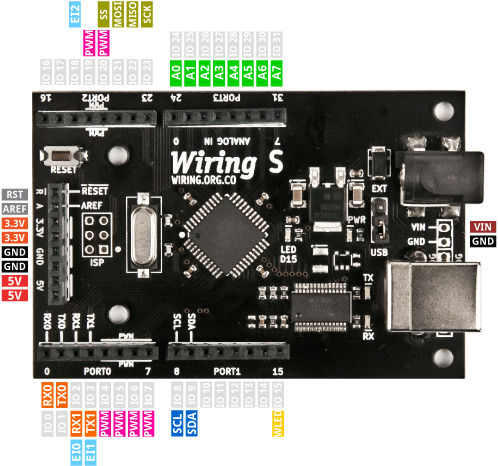
\includegraphics[scale=0.3]{img/wiring}
    \caption{Plataforma para prototipado}
    \label{fig:wiring}
  \end{figure}
\end{frame}

\begin{frame}{FreeRunner}{\url{http://www.openmoko.com}}
  \begin{figure}
    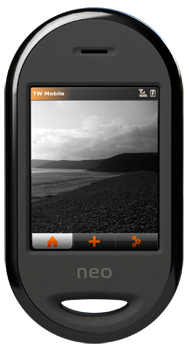
\includegraphics[scale=0.65]{img/freerunner_shop1}
    \caption{Teléfono móvil.}
    \label{fig:openmoko}
  \end{figure}
\end{frame}

\begin{frame}{NanoNote}{\url{https://sharism.cc}}
  \begin{figure}
    \centering
    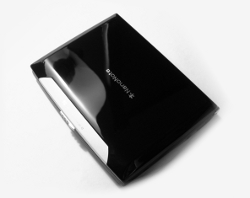
\includegraphics{img/nano}
    \caption{Agenda digital}
    \label{fig:nanonote}
  \end{figure}
\end{frame}

\begin{frame}{ECB AT91 V2}{\url{http://www.emqbit.com}}
  \begin{figure}
    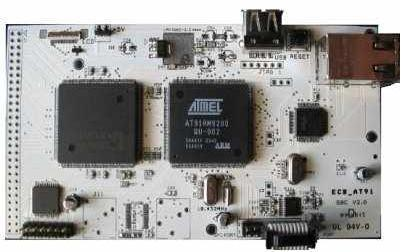
\includegraphics[scale=0.6]{img/V2}
    \caption{Free open SBC design Single Board.}
    \label{fig:ecb}
  \end{figure}
\end{frame}

\section{Software Libre disponible}

\subsection[gEDA - \url{http://www.gpleda.org}]{gEDA}

\begin{frame}{GPL'd Electronic Design Automation}
  \begin{figure}[!h]
    \centering
    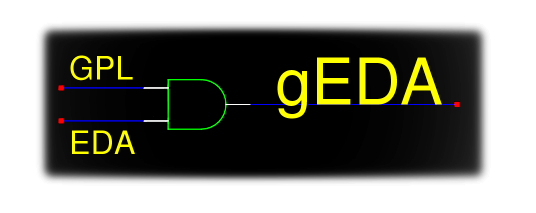
\includegraphics[scale=0.4]{img/geda.png}
  \end{figure}
  \begin{itemize}
  \item gEDA es acrónimo de GPL'd Electronic Design Automation.
  \item gEDA es una suite de aplicaciones de software libre EDA para diseño de circuitos eléctricos, con la que se puede hacer captura esquemática, simulación, creación de prototipos y producción.
  \end{itemize}
\end{frame}

\begin{frame}{Herramientas que componen la suite}
  \begin{itemize}
  \item gEDA / gaf(gschem and friends)
      \begin{itemize}
      \item Captura esquemática.
      \item Librería de símbolos.
      \item Verificador de símbolos.
      \item Editor de atributos.
      \item Generador de netlist.
      \item Utilidades.
      \item Documentación y ejemplos.
      \end{itemize}
    \item Desarrolladas separadamente pero que se usan con la suite.
      \begin{itemize}
      \item Simulación análoga.
      \item Creación de circuitos impresos.
      \item Simulación digital.
      \end{itemize}
  \end{itemize}
\end{frame}

\begin{frame}{gaf - gschem and friends}{gschem}
  \begin{figure}[!h]
    \centering
    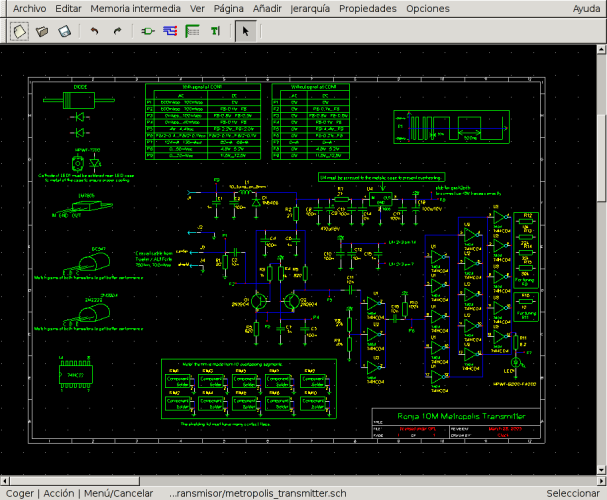
\includegraphics[scale=0.35]{img/gscheme.png}
  \end{figure}

\end{frame}

\begin{frame}{gaf - gschem and friends}{gschem}
  Programa de dibujo especializado para ECAD.
  \begin{itemize}
  \item Entiende conexiones eléctricas.
  \item Asociación de atributos.
  \item Diseño jerárquico.
  \item Programado en C y scheme.
  \end{itemize}
\end{frame}

\begin{frame}{gaf - gschem and friends}{Librería de símbolos}
  \begin{figure}[!h]
    \centering
    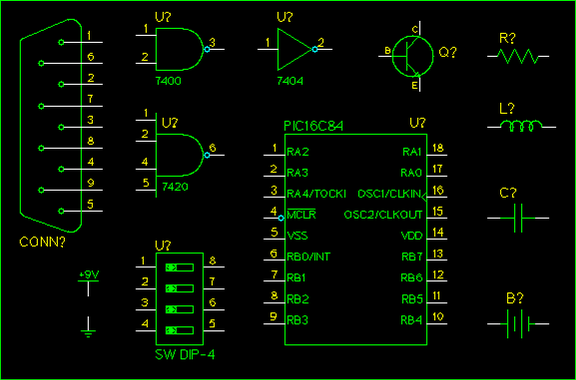
\includegraphics[scale=0.25]{img/simbolos.png}
  \end{figure}
  \begin{itemize}
  \item Más de 1400 símbolos, todos bajo GPL.
  \item El formato de archivo es ASCII, usado para símbolos y esquemas.
  \item Descarga de símbolos \url{http://www.gedasymbols.org}
  \item \textbf{gsymcheck} Verificador de símbolos.
  \end{itemize}
\end{frame}

\begin{frame}{gaf - gschem and friends}{gattrib}
  \begin{figure}[!h]
    \centering
    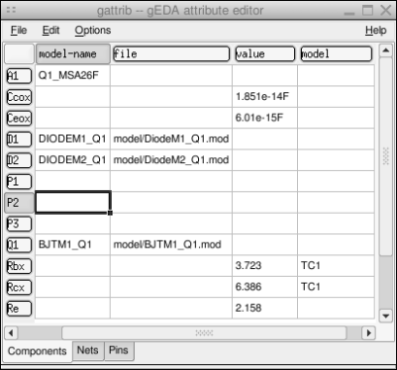
\includegraphics[scale=0.4]{img/gattrib.png}
  \end{figure}
  Editor de Atributos
\end{frame}

\begin{frame}{gaf - gschem and friends}{docs, examples}
  \begin{itemize}
  \item \textbf{gnetlist} Genera apartir de archivo esquemático un netlist en alguno de los 28 formatos soportados.
    \pause
  \item Utilidades: 17 utilidades más que complementan gEDA/gaf (cli).
    \begin{itemize}
    \item gmk\_sym, smash\_megafile, convert\_sym, sarlacc\_schem, olib, gsch2pcb, grenum, gschlas, sarlacc\_sym, gschupdate, gsymupdate, gschemdoc, refdes\_renum, tragesym, pads\_backannotate, garchive, gsymfix.pl
    \end{itemize}
  \end{itemize}
\end{frame}

\begin{frame}{gaf - gschem and friends}{docs, examples}
  \begin{itemize}
  \item Documentación: Manuales de los programas y el wiki completo hasta la fecha de la revisión.
    \pause
  \item Ejemplos:
    \begin{itemize}
    \item gTAG: Interface para conectar desde el puerto USB del computador a dispositivos conm JTAG.
    \item Detector de luz
    \item Amplificador de radio frecuencia
    \item Amplificador en dos etapas
    \end{itemize}
  \end{itemize}
\end{frame}

\begin{frame}{Simulación análoga}{\textbf{gnucap} - \url{http://www.gnu.org/software/gnucap}}
  GNU circuit Analisys Package
  \begin{itemize}
  \item Simulador de circuitos de proposito general.
  \item Aunque soporta modelos de spice no esta basado en spice.
  \end{itemize}
\end{frame}

\begin{frame}{Simulación análoga}{\textbf{ngspice} - \url{http://ngspice.sourceforge.net}}
  \begin{figure}[!h]
    \centering
    
\includegraphics[scale=0.5]{img/nglogo.jpg}
  \end{figure}
  Simulador de circuitos basado en los simuladores de código abierto Spice3f5, Cider1b1 y Xspice.
\end{frame}

\begin{frame}{Simulación análoga}{GSpiceUI}
  \begin{figure}[!h]
    \centering
    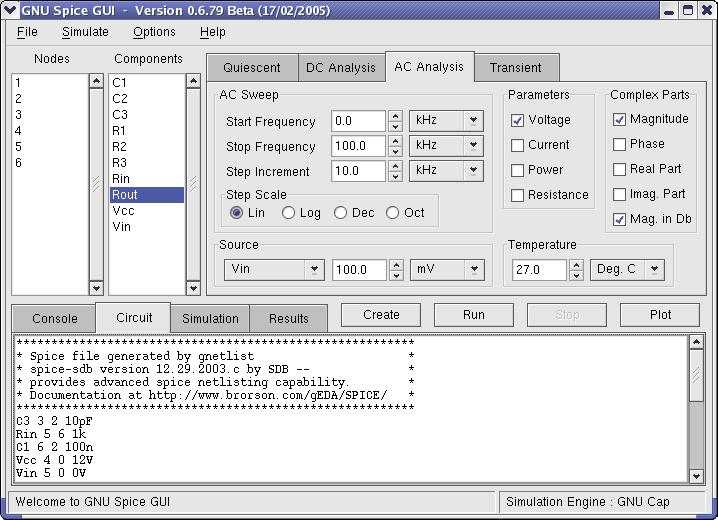
\includegraphics[scale=0.3]{img/GSpiceUI.jpg}
  \end{figure}
  Frontend gráfico para gnucap y ngspice.
\end{frame}

\begin{frame}{Simulación análoga}{\textbf{gwave} - \url{http://gwave.sourceforge.net}}
  \begin{figure}[!h]
    \centering
    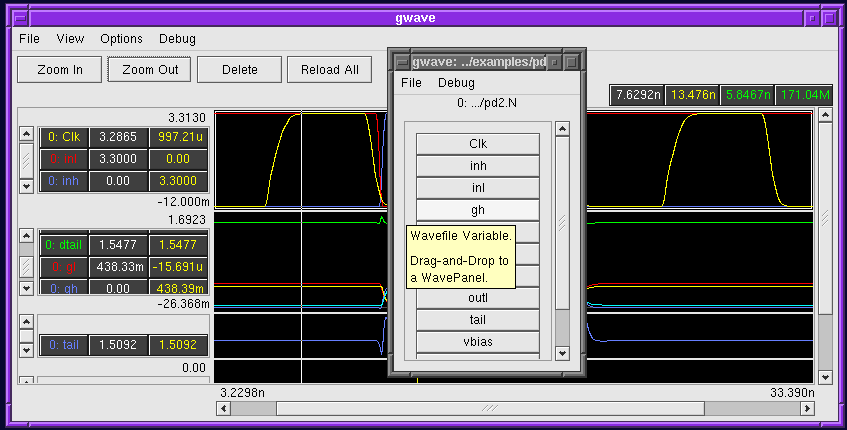
\includegraphics[scale=0.25]{img/gwave.png}
  \end{figure}
  \begin{itemize}
  \item Visor de señales análogas.
  \item Puede leer archivos bianrios (raw) de spice2G6, spice3F5 o ngspice y datos tabulados en formato ASCII para usar con gnucap o cualquier otra herramienta que genere este tipo de archivo.
  \end{itemize}
\end{frame}

\begin{frame}{Creación de circuitos impresos}{xgsch2pcb}
  \begin{figure}[!h]
    \centering
    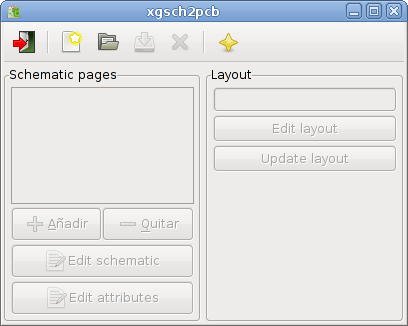
\includegraphics[scale=0.35]{img/xgsch2pcb.png}
  \end{figure}
  Front-end gráfico para generar archivos pcb apartir de un archivo de gschem.
\end{frame}

\begin{frame}{Creación de circuitos impresos}{PCB - \url{http://pcb.gpleda.org}}
  \begin{figure}[!h]
    \centering
    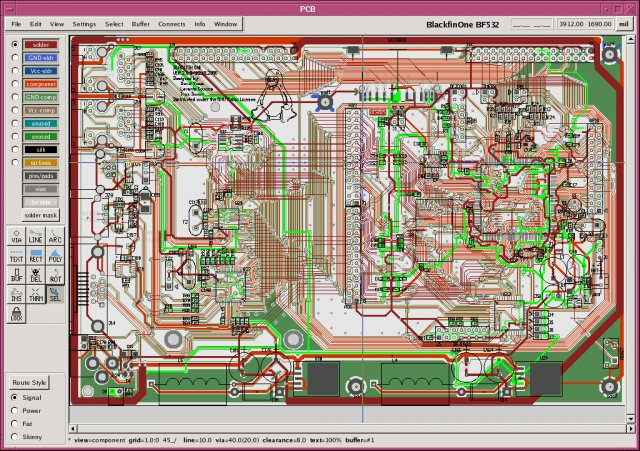
\includegraphics[scale=0.35]{img/pcb.jpg}
  \end{figure}
  Editor de circuitos impresos (PCB).
\end{frame}

\begin{frame}{Creación de circuitos impresos}{Gerbv - \url{http://gerbv.sourceforge.net}}
  \begin{figure}[!h]
    \centering
    
\includegraphics{img/gerbv.png}
  \end{figure}
  Visor de archivos gerber.
\end{frame}

\begin{frame}{Simulación digital}{Icarus Verilog - \url{http://www.icarus.com/eda/verilog}}
  \begin{figure}[!h]
    \centering
    
\includegraphics[scale=0.6]{img/icarus.png}
  \end{figure}
  \textbf{iverilog} Herramienta de simulación y síntesis para el lenguaje de descripción de hardware Verilog HDL.
\end{frame}

\begin{frame}{Simulación digital}{\textbf{gtkwave} - \url{http://gtkwave.sourceforge.net}}
  \begin{figure}[!h]
    \centering
    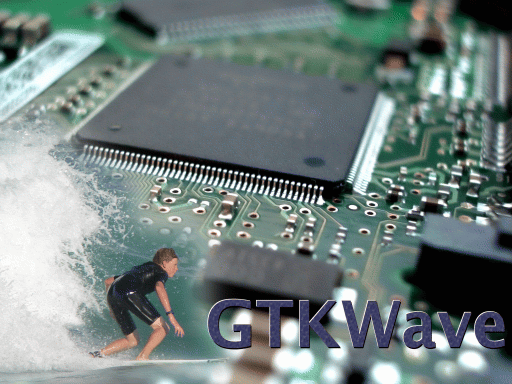
\includegraphics[scale=0.25]{img/gtkwave.png}
  \end{figure}
  \begin{itemize}
  \item Visor de señales digitales.
  \item Formatos soportados: VCD, EVCD,	LXT, Synopsis y .out.
  \end{itemize}
\end{frame}

\subsection[qucs - \url{http://qucs.sourceforge.net}]{qucs}

\begin{frame}{Quite Universal Circuit Simulator}
  \begin{figure}
    \centering
    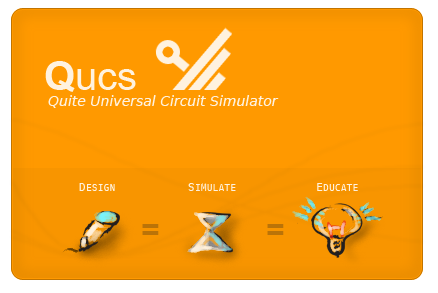
\includegraphics[scale=0.4]{qucs/img/qucslogo4.png}
  \end{figure}
  Simulador de circuitos integrado, lo que significa que puede configurar un circuito eléctrico con un interfaz gráfico y simular su comportamiento en pequeña señal, gran señal y con ruido.
\end{frame}

\subsection[kicad - \url{http://kicad.sourceforge.net}]{kicad}

\begin{frame}{¿Qué es kicad?}
  \begin{figure}[!h]
    \centering
    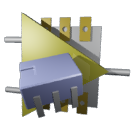
\includegraphics[scale=0.5]{img/kicad.png}
  \end{figure}
  Diseño y fabriacación de circuitos impresos
  Se compone de un gestor de proyectos y cuatro programas principales.
\end{frame}

\begin{frame}{Componentes}
  \begin{figure}[!h]
    \centering
    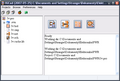
\includegraphics[scale=0.6]{img/kicad-project.png}
    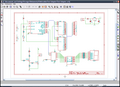
\includegraphics[scale=0.5]{img/eeschema.png}
    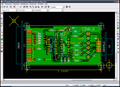
\includegraphics[scale=0.5]{img/pcbnew.png}
    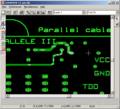
\includegraphics[scale=0.4]{img/gerbview.png}
  \end{figure}
  \begin{itemize}
  \item \alert{kicad} El gestor de proyectos
  \item \alert{eeschema} Capturador esquemático
  \item \alert{cvpcb} Selector de componentes usados en el diseño del circuito
  \item \alert{pcbnew} Editor de circuitos impresos
  \item \alert{gerbview} Visor Gerber (Documentos Fotoploter)
  \end{itemize}
\end{frame}

% \begin{frame}{kicad}{El selector de componentes usados en el diseño del circuito}
%   \textbf{cvpcb} Es una herramienta que permite asignar huellas/formas (footprint) de circuito impreso a los símbolos esquemáticos del diseño en eeschema.
% \end{frame}

\subsection[\LaTeX - \url{http://www.latex-project.org}]{\LaTeX}

\begin{frame}{\LaTeX}
  \begin{figure}
    \centering
    
\includegraphics[scale=0.6]{img/latex}
  \end{figure}
  \begin{itemize}
  \item Documentación estructurada (WYSIWYM - What You See Is What You Mean)
  \item Paquetes especializados
    \begin{itemize}
    \item Mapas de karnaugh
    \item Formatos IEEE
    \item Esquemas de circuitos
    \item Muchos más\dots
    \end{itemize}
  \end{itemize}
\end{frame}

\subsection[Octave - \url{http://www.octave.org}]{Octave}

\begin{frame}{¿Qué es octave?}
  \begin{figure}
    \centering
    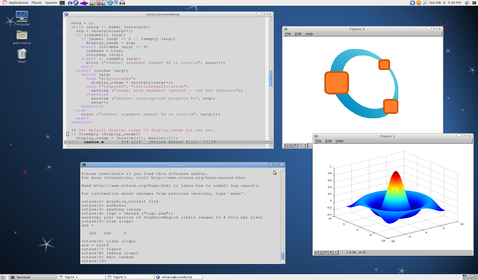
\includegraphics[scale=0.5]{img/octave}
  \end{figure}
  Software para análisis númerico
\end{frame}

\subsection[Scilab - \url{http://www.scilab.org}]{Scilab}

\begin{frame}{¿Qué es scilab?}
  \begin{figure}
    \centering
    
\includegraphics{scilab/img/Scilab-WebSite.png}
    
\includegraphics{scilab/img/Puffin-Logo_medium}
  \end{figure}
  Software para computación numérica con centenares de funciones matemáticas, un lenguaje de programación de alto nivel desde el que se puede acceder a estructuras de datos avanzadas y capacidad para graficar en 2D y 3D.
\end{frame}

\begin{frame}{¿Para qué scilab?}
  \begin{figure}
    \centering
    
\includegraphics{scilab/img/Scilab-WebSite.png}
    
\includegraphics{scilab/img/Puffin-Logo_medium}
  \end{figure}
  \begin{itemize}
  \item Matemáticas y simulación
  \item Visualización 2D y 3D
  \item Optimización
  \item Estadística
  \item Análisis y diseño de sistemas de control
  \item Procesamiento de señales
  \item Desarrollo de aplicaciones
  \end{itemize}
\end{frame}

\section{Análisis transitorio}


\begin{frame}{xcos}
  Editor gráfico para diseñar modelos de sistemas dinámicos híbridos.
  \begin{figure}
    \centering
    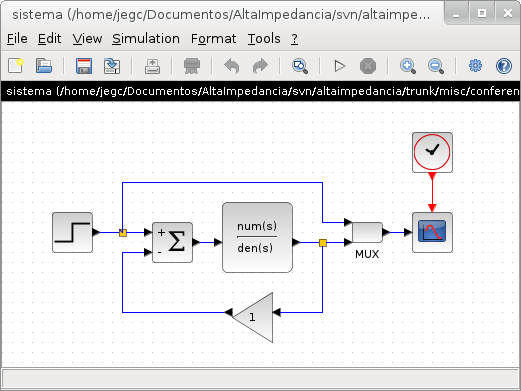
\includegraphics[scale=0.6]{scilab/img/xcos.png}
  \end{figure}
\end{frame}

\subsection{Oscilador Colpitts}

\begin{frame}{qucs}
  \begin{figure}
    \centering
    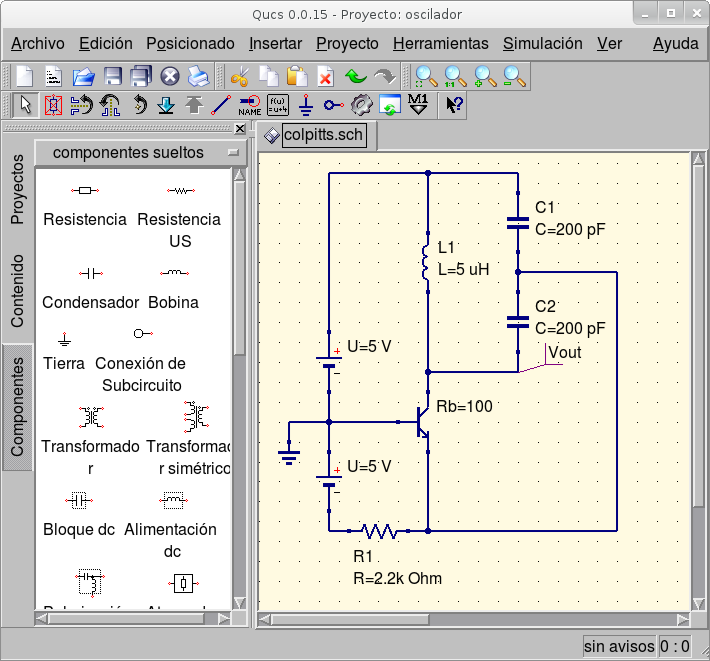
\includegraphics[scale=0.3]{qucs/img/qucs-colpitts.png}
  \end{figure}
\end{frame}

\begin{frame}{gschem}
  \begin{figure}
    \centering
    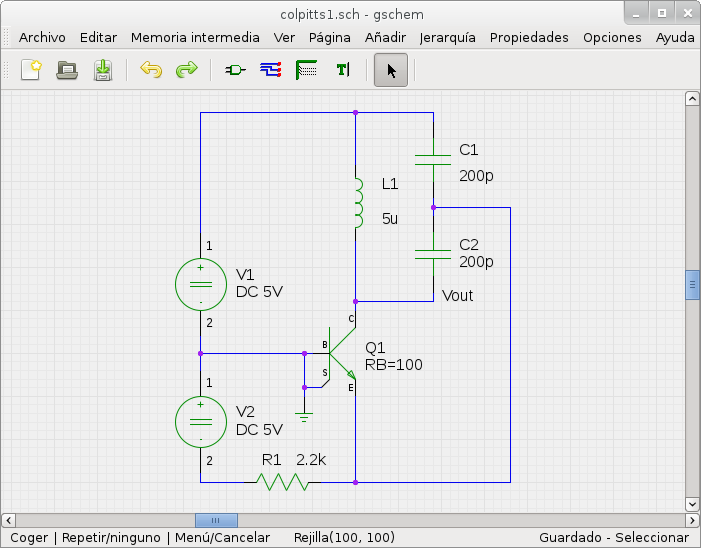
\includegraphics[scale=0.4]{geda/img/gschem/gschem-colpitts.png}
  \end{figure}
\end{frame}

\section{Análisis en frecuencia}

\subsection{Filtro pasa altos}

\begin{frame}{qucs}
  \begin{figure}
    \centering
    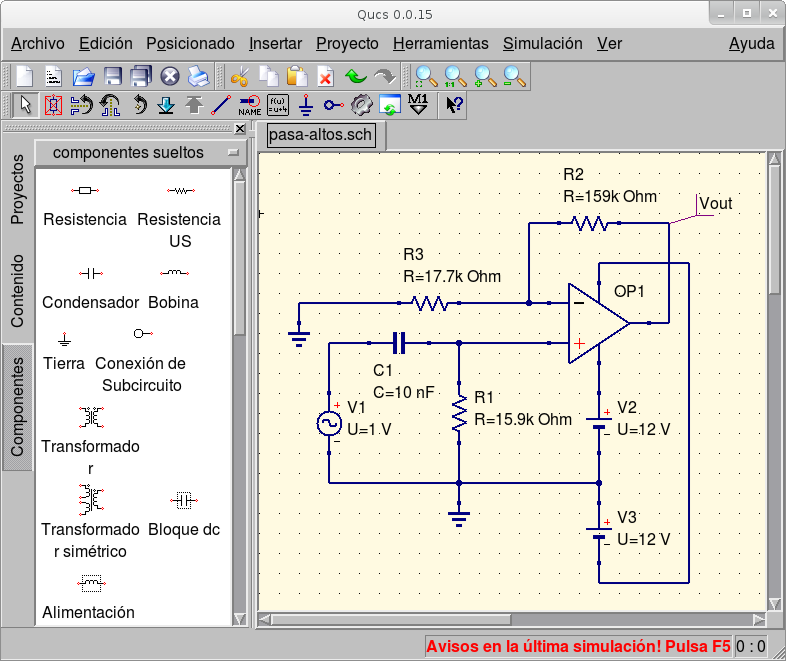
\includegraphics[scale=0.4]{qucs/img/qucs-pasaltos.png}
  \end{figure}
\end{frame}

\begin{frame}{gnucap}
  \begin{figure}
    \centering
    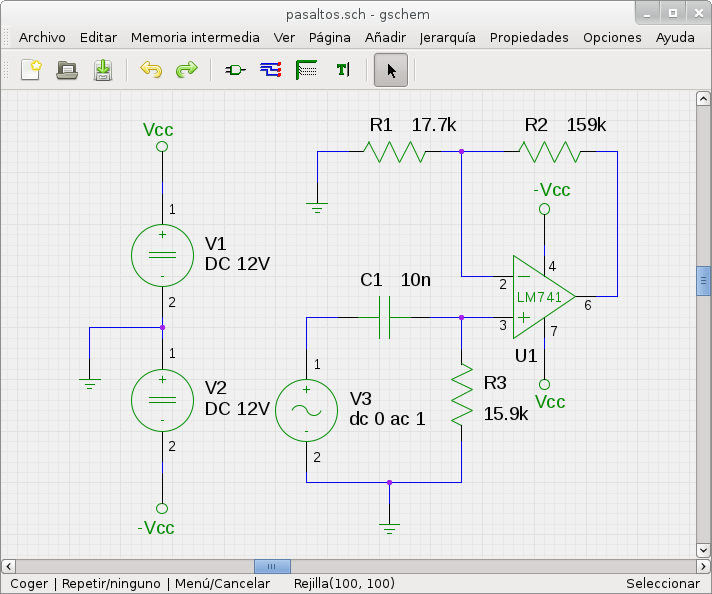
\includegraphics[scale=0.4]{geda/img/gschem/gschem-pasaltos.png}
  \end{figure}
\end{frame}


\section<presentation>*{Simulación de circuitos con Software Libre}

\begin{frame}{¿Que tiene que ver Debian en esta charla?}
  \begin{figure}
    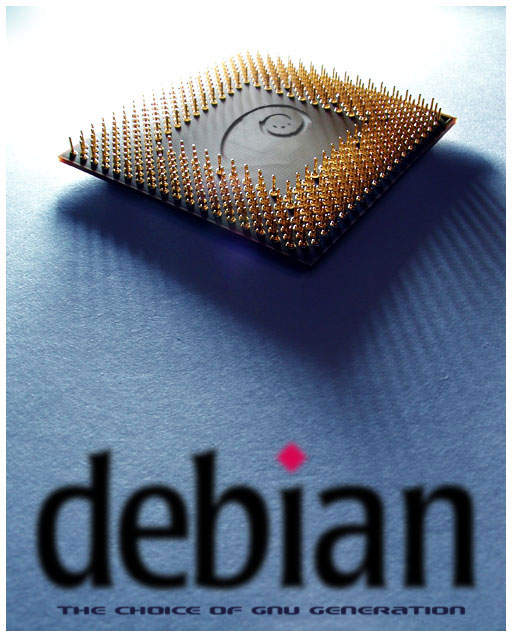
\includegraphics[scale=0.32]{img/choice.jpg}
  \end{figure}
    \begin{itemize}
  \item También existe FEL
  \end{itemize}
\end{frame}

\begin{frame}{Conclusiones}
  \begin{block}{}
    \begin{itemize}
    \item Hay Software Libre variado para hacer simulaciones de circuitos por lo menos en el ámbito académico de una universidad.
    \item A veces es necesario usar más de un programa para lograr una simulación de un solo circuito, esto a primera vista puede parecer compicado, pero en realidad termina siendo una ventaja pues es posible hacer un análisis más profundo si con una sola aplicación no se obtiene el resultado deseado.
    \end{itemize}
  \end{block}
\end{frame}

\begin{frame}{Agradecimientos}
  \begin{itemize}
  \item A todos los maestros que durante la carrera me permitieron hacer la tarea con software libre y a los que no también porque apredí más, tuve que hacerla dos veces ;)
  \item Todas las personas que han hecho parte de los colectivos en los que hemos trabajado en este tema.
  \end{itemize}
\end{frame}

\appendix

\section<presentation>*{Referencias}

\begin{frame}
  \frametitle<presentation>{Bibliografía I}
  \begin{thebibliography}{99}
    \beamertemplatebookbibitems
  \bibitem[1]{Savant}C. J. Savant, Jr., Martin S. Roden y Gordon L. Carpenter
    \newblock \emph{DISEÑO ELECTRÓNICO Circuitos y sistemas}
    \newblock Addison Wesley Longman, 1992
  \end{thebibliography}
\end{frame}

\begin{frame}[allowframebreaks]
  \frametitle<presentation>{Infografía}
  \begin{thebibliography}{99}
    \beamertemplatearticlebibitems
  \bibitem<1->[Xcos en images]{video} \emph{Xcos en images}, \url{http://www.youtube.com/watch?v=nKSvAX9D1Vc}
    \newblock 15 de septiembre de 2011
  \bibitem<1->[Oscilador colpitts]{colpitts}\emph{Oscilador del ejemplo} \url{http://qucs.sourceforge.net/examples/colpitts_base.sch}
    \newblock 15 de septiembre de 2011
  \end{thebibliography}
\end{frame}

\section<presentation>*{Sobre este documento}

\begin{frame}
  \begin{block}{Licencia}
    \begin{figure}
      
\includegraphics[scale=0.9]{img/by-sa}
    \end{figure}
    \centering
    \small Creative Commons\\
    \small Atribución-Compartir Obras Derivadas Igual 2.5 Colombia\\
    \small \url{http://creativecommons.org/licenses/by-sa/2.5/co}
\end{block}
\begin{block}{}
  Creado con \LaTeX / Beamer
\end{block}
\end{frame}

\section<presentation>*{Comunidades}

\begin{frame}{Como unirse}
  \begin{figure}
    
\includegraphics{img/altaimpedancia-acerca-de}
  \end{figure}
  \begin{block}{}
    \begin{itemize}
    \item Linux en Caja - \url{http://linuxencaja.net}
    \item HackBo - \url{http://hackbo.co}
    \end{itemize}
  \end{block}
  \begin{block}{Contacto}
    \centering
    Jorge Ernesto Guevara Cuenca\\
    \href{mailto:ernesto@altaimpedancia.org}{ernesto@altaimpedancia.org}\\
  \end{block}
\end{frame}

\end{document}
%@-leo
